\chapter{Results}
\label{chapter:results}

\section{Uncertainties}
\label{sec:uncertainties}

\subsection{Statistical Uncertainties}
\label{ssec:stat_uncertainty}

The statistical uncertainties due to the number of data events are propagated
through the unfolding method, as discussed in
\SEC~\ref{ssec:unfolding_statistical_uncertainties}. This uncertainty is
generally around 0.3\% for both the normalized and absolute cross section
measurement, but reaches 1.2\% in the highest \phistar bins. It is one of the
dominant uncertainties for the normalized cross section measurements.

\subsection{Statistical Uncertainties from the Monte Carlo Samples}
\label{ssec:mc_stat_uncertainty}

The \MADGRAPH signal MC sample has fewer events which pass our final selection
than there are data events. As this sample is used to unfold the data, its
statistical uncertainty affects the final measurement.

The affect of the statistical uncertainty on the bin migration matrix is
propagated through the use of toy MC, detailed in
\SEC~\ref{ssec:unfolding_statistical_uncertainties}. The uncertainty found with
this method is about 0.1 to 0.2\% for both the normalized and absolute cross
section measurement.

In addition to affecting the unfolding, the low number of events in the MC
affects the efficiency correction discussed in \SEC~\ref{ssec:eff_correction}
and shown in \FIG~\ref{fig:average_efficiencies}. These uncertainties are about
0.3\%, but rise to 1.4\% in the highest \phistar bins.

These two sources of uncertainty are measured separately. The finally
uncertainty due to the statistical uncertainties from the \MADGRAPH signal MC
sample is the sum in quadrature of both sources.

\subsection{Luminosity Uncertainty}
\label{ssec:lumi_uncertainty}

The integrated luminosity is measured at CMS by using the occupancy in the
pixel detector during minimum-bias events \cite{cms_lumi_2013}. This luminosity
measurement is calibrated by using van der Meer scans---a method in which the
two beams are displaced and then ``swept'' across each other as the offset is
reduced \cite{vandermeer_1968}.

The integrated luminosity for the run period considered in this analysis is
known to 2.6\%. This uncertainty taken to be fully correlated bin-by-bin in
\phistar for the absolute cross section measurement, and so is the dominant
uncertainty. The luminosity cancels in the normalized measurement and so the
uncertainty only affects the background subtraction, but this contribution is
negligible compared to the background subtraction uncertainty (discussed in
\SEC~\ref{ssec:background_subtraction_uncertainty}). This calculation of the
luminosity is the primary motivation behind making a normalized cross section
measurement.

\subsection{Pileup Uncertainty}
\label{ssec:pileup_uncertainty}

As discussed in \SEC~\ref{ssec:monte_carlo}, the high beam intensity at the LHC
leads to multiple proton-proton interactions at each bunch crossing. This is
modeled in MC by overlaying multiple simulated minimum-bias events on top of
each simulated event. The distribution of pileup in MC is reweighted to match
the data distribution based on the calculated instantaneous luminosity and the
inelastic proton-proton cross section. The uncertainty due to this reweighting
process is calculated by varying the inelastic cross section by plus and minus
5\%, recalculating the data distribution of pileup, and reweighting to the MC
samples to match this new distribution. The full analysis is then performed
with these MC samples and the differences between the \phistar distributions is
taken as a systematic uncertainty. The pileup uncertainty for the absolute
cross section measurement is around 0.2 to 0.5\%, while the uncertainty for the
normalized cross section measurement is between 0 and 0.7\%.

\subsection{Background Subtraction Uncertainty}
\label{ssec:background_subtraction_uncertainty}

The background subtraction is discussed in \SEC~\ref{sec:background}. There are
three categories of backgrounds, and the uncertainty in each category is
determined with a different method. The uncertainties for all three categories
are added in quadrature.

The first category consists of the various backgrounds with two independent
decay chains: $\ttbar$, $\W\W$, $\DYtotautau$, $t\W$, and $\tbar\W$. The
contributions from these backgrounds are estimated by using an \emu control
sample as discussed in \SEC~\ref{ssec:emu_sample}. The uncertainty from the
scale factors derived using this method are propagated through to the final
result using 500 toy MC variations. For each variation, the scale factors are
randomly drawn from a Gaussian distribution with mean equal to the nominal
value of that scale factor and width equal to the uncertainty on the scale
factor. Each toy is then used to weight the background samples, the subtraction
is performed, and the full analysis is performed with the newly subtracted data
sample. The uncertainty due to the subtraction of this category of background
for each bin in \phistar is defined by the spread of the central 68.2\% values
obtained by this method.

The second category consists of the backgrounds with a real \Z boson: $\Z\Z$
and $\W\Z$. For these samples, the uncertainty is calculated by taking a
correlated 20\% uncertainty on the theoretical cross section.

The third and final category consists of the \QCDjets and \wjets
backgrounds. The method of estimating this background is discussed in
\SEC~\ref{ssec:qcd_background}. Instead of using the uncertainties from the
fit, which would not account for any systematics in the method used, a
conservative 100\% uncertainty is used.

The uncertainty due to the background subtraction for both the absolute and
normalized cross section measurements ranges from about 0.03 to 0.59\%, with
the higher values in the highest \phistar bins.

\subsection{\texorpdfstring{\pt}{PT} Scale Uncertainty}
\label{ssec:pt_scale_uncertainty}

One of the advantages of the \phistar variable is that it does not use the
momentum of the electrons and instead uses only the angles between them. This
makes \phistar less sensitive to any potential problems with the \pt
measurement of electrons.

However, the measurement of the \pt of the electrons is used to determine which
events are included in our sample. Therefore, a shift in the \pt scale of the
detector will either add or remove events that have electrons near the \pt
selection requirement boundaries. To determine the uncertainty due to the \pt
scale, we vary the \pt values of all of the electron up and down by 0.3\%.
\TODO{The largest difference in each \phistar bin between the nominal result
    and the results with the modified \pt scale is taken as the uncertainty in
that bin.} The uncertainty due to the \pt scale for the absolute cross section
measurement is 0.08 to 0.17\%, while the uncertainty for the normalized cross
section measure is 0 to 0.10\%.

\subsection{Trigger, Reconstruction, and Identification Scale Factors Uncertainty}
\label{scale_factor_uncertainty}

Differences between the MC and data are corrected for using scale factors.
Three different sets of scale factors are used to reweight the MC samples:
trigger scale factors (discussed in \SEC~\ref{ssec:sf_trigger}), reconstruction
scale factors (discussed in \SEC~\ref{ssec:sf_reconstruction}), and
identification scale factors (discussed in \SEC~\ref{ssec:sf_id}).

In all three cases, the uncertainties on the scale factors are propagated
through to the final measurement using 500 toy MC variations. In this method,
every toy is constructed by drawing each scale factor from a Gaussian
probability distribution with its mean set to nominal value of the scale factor
and its width set to the quadrature sum of the uncertainties on the scale
factor. Each toy is then used to weight the MC samples used in this analysis,
and the full analysis is performed with that newly weighted sample. The
uncertainty on the final result due to one of the three types of scale factors
is taken to be defined by the central 68.2\% of results from the toys.

This procedure for propagating the uncertainty is performed independently for
each of the three types of scale factors. The total uncertainty due to the
scale factors is the quadrature sum of the three results. The uncertainty is
small, $\le 0.02\%$, for both the absolute and normalized cross section
measurements.

\subsection{Electron Angular Position Uncertainty}

Since \phistar depends on the angles between the two electrons, it is sensitive
to mismeasurement of these angles. As discussed in
\SEC~\ref{sec:electron_reconstruction}, the position of a reconstructed
electron comes from the tracker, and therefore misalignment of the tracker
would lead to a systematic uncertainty on the angle measurement. The magnitude
of this systematic is estimated by using the position of the ECAL supercluster
associated with the electron to calculate the electron's position instead of
using the track. The new supercluster-only position is then used to calculate a
new \phistarSC that does not depend on the alignment of the tracker.

The position of the supercluster does not take into account the amount the
bending of the electron due to the magnetic field. While $\eta$ is unchanged by
the pretense of the field, $\phi$ is changed. A correction is applied to $\phi$
to find the angle at the interaction point, $\phizero$, based on the angle of
the supercluster, $\phisc$. This correction is given by
\EQ~\ref{eq:b_field_correction} where $q$ is the charge of the electron, \pt is
the transverse momentum of the electron, $B$ is the magnitude of the magnetic
field, and \Reffective is the effective radius of ECAL as a function of $\eta$
and $\theta$ as given in \EQ~\ref{eq:effective_radius}. The charge and momentum
come from the electron matched to the supercluster, and although they are
determined in combination with the tracker, they are far less susceptible to
the small scale misalignments of the tracker that we are considering.

\begin{equation}\label{eq:b_field_correction}
    \sin \left( \phisc - \phizero \right)
    =
    - \Reffective \frac{q B}{2 \pt}
\end{equation}

\begin{equation}\label{eq:effective_radius}
    \Reffective
    =
    \left\{
        \begin{array}{ll}
            1.29 \meters & \text{if } |\eta| < 1.4442 \\
            3.14 \meters \times \tan \left(\coord{\theta}\right) & \text{otherwise}
        \end{array}
    \right.
\end{equation}

The resulting \phistarSC distribution is compatible within statistical
uncertainties with the \phistar distribution and so no systematic uncertainty
is assigned for the angular position.

\TODO{Plot of \phistar vs \phistarSC?}

\subsection{Uncertainty from Four Vector Corrections}

The \mee distribution in the \MADGRAPH signal MC sample does not precisely
match the distribution in data, as seen in \FIG~\ref{fig:z_mass}. This
discrepancy remains even after applying the various energy and momentum
corrections to the electrons. In order to determine what effect this has on the
final measurement, the \MADGRAPH signal MC sample is reweighted to remove this
difference. The ratio between the nominal \phistar value and the value derived
after this reweighting is shown in \FIG~\ref{fig:z_mass_reweighted}. The
circular points show the ratio of the reconstructed \phistar distributions,
while the square points show the ratio of the generated \phistar distributions.
The errors are binomial. Most of the points are consistent with \num{1}, and so
systematic uncertainty is assigned for this disagreement.

\begin{figure}[!htbp]
    \centering
    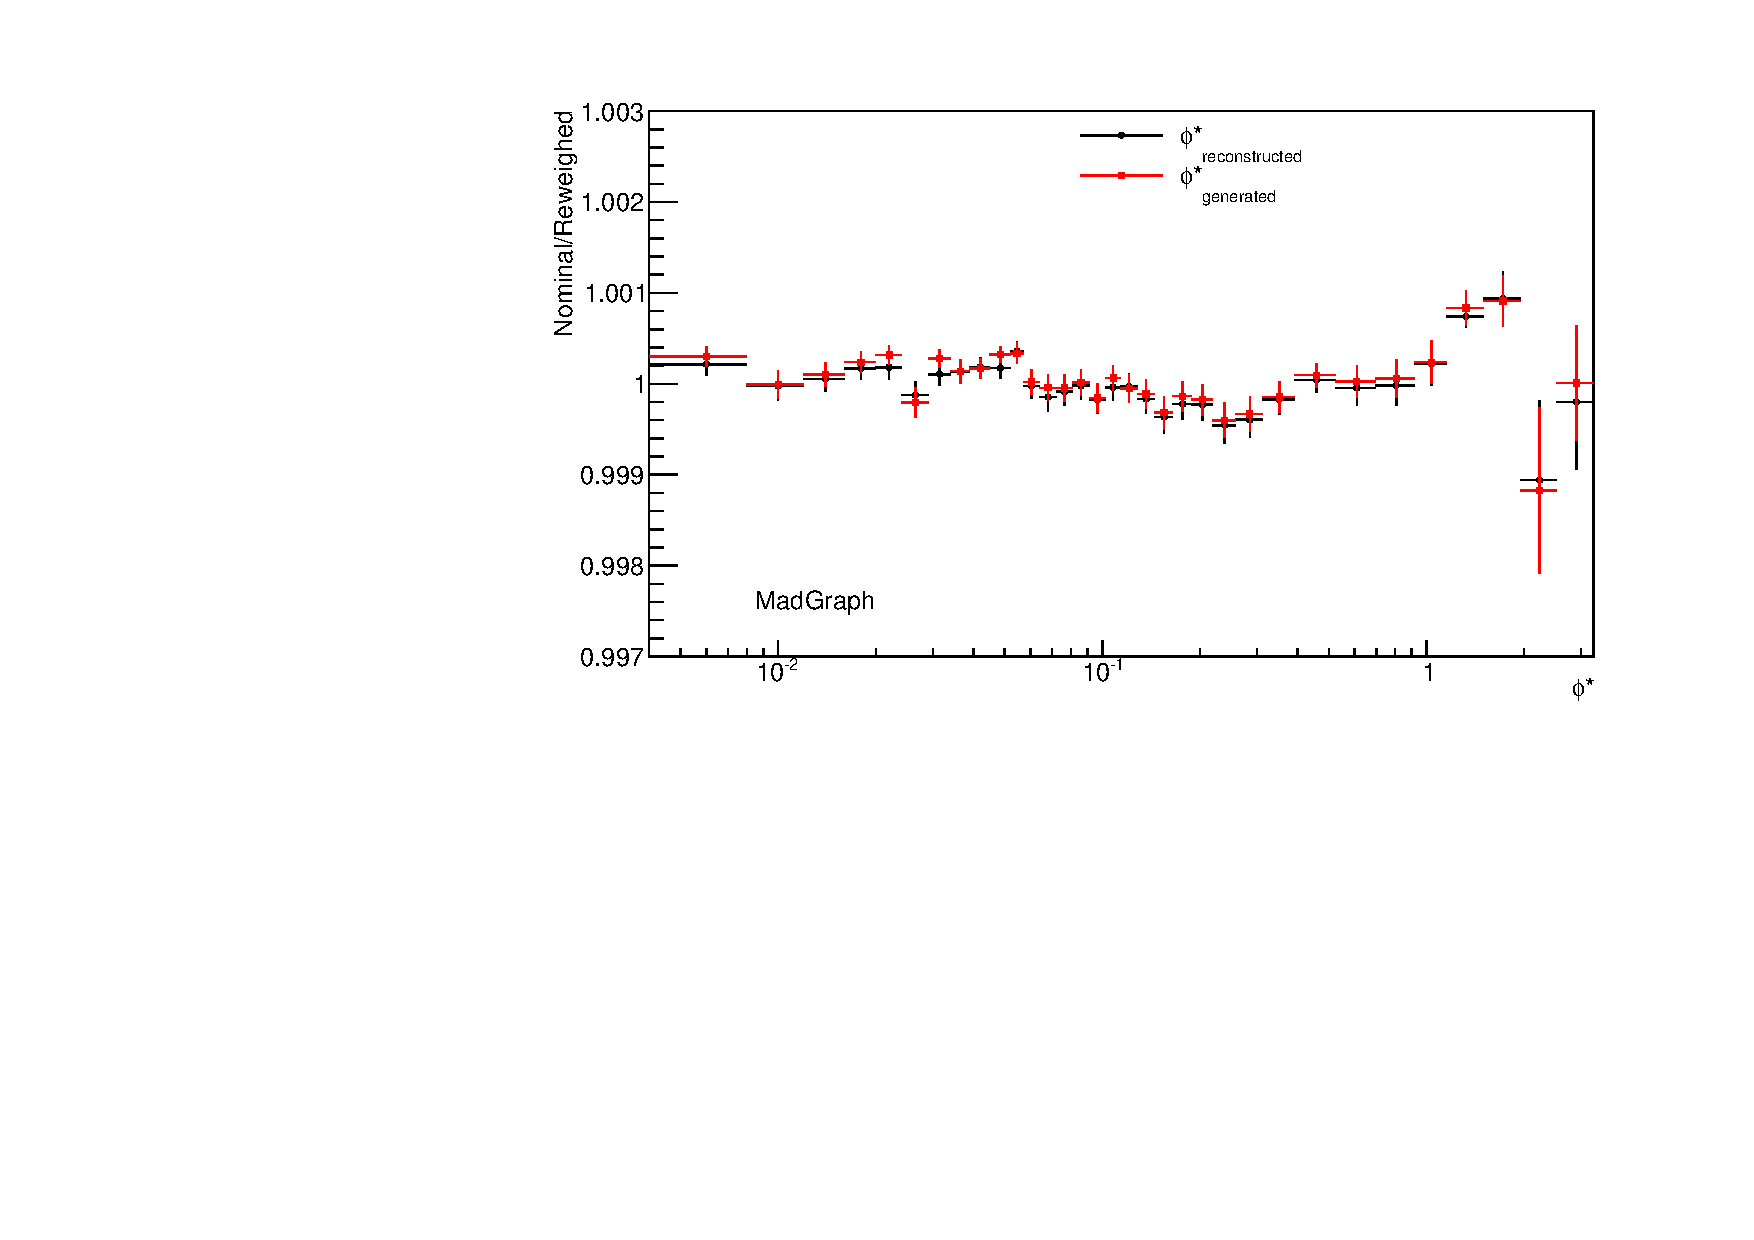
\includegraphics[width=\textwidth]{figures/ZMass_reweighed.pdf}
    \caption[
        The ratio of \phistar in \MADGRAPH before and after reweighting to
        remove the differnce in the \mee distribution between MC and data.
    ]{
        The ratio of \phistar in \MADGRAPH before and after reweighting to
        remove the difference in the \mee distribution between MC and data seen
        in \FIG~\ref{fig:z_mass}. The circular points are this ratio in the
        reconstructed quantity, while the square points are this ratio in the
        generated quantity. The uncertainties are binomial.
    }
    \label{fig:z_mass_reweighted}
\end{figure}
